\documentclass[conference]{IEEEtran}
\IEEEoverridecommandlockouts

\usepackage{cite}
\usepackage{amsmath,amssymb,amsfonts}
\usepackage{graphicx}
\usepackage{textcomp}
\usepackage{xcolor}
\usepackage{tikz}
\usepackage{url}
\usepackage{graphicx}
\usepackage{subcaption}
\usetikzlibrary{arrows.meta,positioning,calc}

\def\BibTeX{{\rm B\kern-.05em{\sc i\kern-.025em b}\kern-.08em
    T\kern-.1667em\lower.7ex\hbox{E}\kern-.125emX}}

% Helper command for image placeholders
\newcommand{\imgbox}[2]{%
  \fbox{\parbox{0.93\columnwidth}{\centering\vspace{#1}%
    {\small\sffamily\bfseries IMAGE PLACEHOLDER}\\[2pt]%
    {\scriptsize\sffamily #2}\vspace{#1}}}%
}

\begin{document}

\title{LLM-Based Knowledge Graph Construction and Retrieval for Legal Document Analysis}

\author{\IEEEauthorblockN{Samuel Bag\'{i}n, Marek Van\v{c}o}
\IEEEauthorblockA{\textit{Faculty of Electrical Engineering and Information Technology} \\
\textit{Slovak University of Technology}\\
Bratislava, Slovakia \\
xbagins@stuba.sk, marek\_vanco@stuba.sk}
}

\maketitle

\begin{abstract}
Legal documents combine long, deeply structured text with numeric tables and references to paragraphs, which makes them difficult to process using classical retrieval-augmented generation. This work presents a pipeline that transforms Slovak financial law into a navigable knowledge graph and answers natural language questions over it. The philosophy of the paper is that legal reasoning rarely depends on a single passage. Instead, it follows chains of concepts such as law, paragraph and obligation. A knowledge graph makes these chains explicit and allows an agent to walk them step by step. We combine layout-aware preprocessing, an ontology-guided extraction stage inspired by ODKE+, and a retrieval stage with an agent inspired by ARK-V1, all orchestrated inside a three-stage KG-GPT pipeline. The result is a system that grounds every answer in explicit graph evidence.
\end{abstract}

\begin{IEEEkeywords}
knowledge graph, large language models, legal document analysis, GraphRAG, information extraction
\end{IEEEkeywords}

\section{Introduction}

With the growing use of Large Language Models (LLMs) across various domains, there is an increasing need for effective methods to analyze and process specific document types. Slovak legal and financial documents are long, heavily structured and full of cross-references. A typical act contains nested paragraphs, numbered items, tables and formulas that describe how to compute a tax. A lawyer or ordinary person who wants to answer a question, such as "which paragraph defines a given obligation" or "how a tax base is calculated", has to follow a chain of references across several pages. Classical retrieval-augmented generation (RAG) over plain text performs poorly in this setting. A single chunk rarely contains the full answer, and the model loses the structural information that paragraphs and tables carry. LLMs alone often struggle with the complex structures and relationships in legal documents, leading to hallucinations and limitations in providing precise information~\cite{yao2024}.

This paper describes a complete pipeline that turns such documents into a knowledge graph (KG) stored in Neo4j~\cite{neo4j} graph database and then queries the graph with a large language model (LLM) agent. The construction phase is inspired by ODKE+~\cite{odkeplus2025}, which uses an ontology to guide open-domain extraction. The query phase uses the three-stage {KG-GPT framework}~\cite{kggpt2023} and plugs an agent inspired by {ARK-V1}~\cite{arkv12025} into its middle stage. The orchestration layer is built on top of LangChain~\cite{langchain} and uses several LLMs for different tasks, such as GPT-5.4-mini, Gemini 2.5 Flash and Pro models.

The main contributions are a preprocessing stage that detects tables and formulas with a document layout detector, a three-step extraction stage that produces a stable legal ontology, and a retrieval stage that walks the graph in small verifiable steps instead of generating a single complex Cypher query. The rest of the paper follows: Section~II reviews related work, Section~III describes document processing, Section~IV describes search and retrieval, and Section~V conclusion.

\section{State of the Art}
Building knowledge graphs from text has traditionally relied on pipelines of specialized NER and relation extraction modules, but recent work increasingly turns to LLMs to carry out the entire extraction end-to-end. The GraphRAG approach of {Edge et al.}~\cite{edge2024} demonstrated that a knowledge graph built by an LLM, combined with community summarization, outperforms classical RAG on query-focused summarization. However, their graphs are extracted in an open-domain fashion and the schema is not explicitly controlled, which is a problem for legal text where the ontology must be stable and auditable. ODKE+~\cite{odkeplus2025} addresses this by combining open-domain detection with an ontology and a schema-driven extraction step. To improve fidelity, KnoBuilder~\cite{knobuilder2025} utilizes an iterative agentic loop featuring planning and self-refining modules, while GraphJudge~\cite{graphjudge2025} employs a discriminative judge to enhance the quality of generated triples and achieves state-of-the-art performance across multiple datasets. On the retrieval side, KG-GPT~\cite{kggpt2023} proposes a three-stage framework of segmentation, retrieval, and inference. ARK-V1~\cite{arkv12025} fills the gap with an iterative agent that repeatedly selects relations and advances anchors to neighbors, ensuring every reasoning hop is explicit and auditable. This mirrors the discrete decision-making in {Reasoning with Trees (RwT)}~\cite{rwt2025}, which utilizes Monte Carlo Tree Search—balancing exploration and exploitation via the UCB formula—to navigate complex paths. For dynamic data, GMeLLo~\cite{gmello2024} translates natural language into SPARQL, while LightRAG~\cite{lightrag2024} provides cost-efficient dual-level search. Additionally, LEGO-GraphRAG~\cite{legograph2024} decomposes the GraphRAG retrieval workflow into modular components (subgraph extraction, path filtering, and path refinement). LLM security and privacy considerations studied in {Security and Privacy Challenges of Large Language Models}~\cite{das2024} also matter in the legal domain, where hallucinated citations can have practical consequences. Grounding every answer in explicit graph evidence is one way to mitigate this risk, and it is one of the main motivations for the architecture proposed here.

\section{Document Processing}

Document processing transforms a raw PDF of a Slovak law into a populated knowledge graph. It has three sub-stages: preprocessing, extraction and database insertion. Fig.~\ref{fig:process} illustrates the process pipeline.

\begin{figure}[h]
\centering
\scalebox{0.8}{%
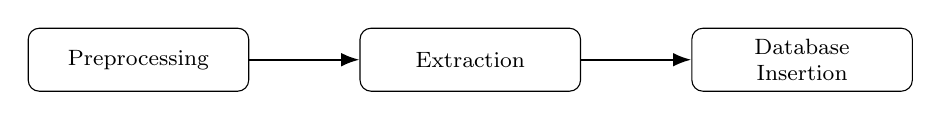
\begin{tikzpicture}[
  node distance=14mm,
  box/.style={draw, rounded corners, minimum height=8mm, minimum width=28mm, align=center, font=\footnotesize},
  arr/.style={-Latex, thick}
]
  \node[box] (pre) {Preprocessing};
  \node[box, right=of pre] (ext) {Extraction};
  \node[box, right=of ext] (db) {Database\\Insertion};
  \draw[arr] (pre) -- (ext);
  \draw[arr] (ext) -- (db);
\end{tikzpicture}
}
\caption{Process pipeline.}
\label{fig:process}
\end{figure}

\subsection{Preprocessing}

Raw PDF text extraction is not enough for legal documents. Tables, for instance, span across several pages and carry hierarchical information (section, chapter, item) that is destroyed if the table is read as free text. Isolated formulas are also frequent and should be kept as image regions rather than fed into a text splitter as garbled characters.

The preprocessing stage converts each page of the PDF into an image at 200~DPI and applies a document layout detector based on the DocLayout-YOLO model. The detector is configured to recognise five target classes: \textit{table}, \textit{picture}, \textit{figure}, \textit{isolate\_formula} and \textit{formula\_caption}. Detections with confidence below $\tau=0.3$ are discarded. For every retained detection the bounding box is cropped from the page image and saved as a PNG file. Consecutive table detections on neighbouring pages are grouped together so that multi-page tables are kept as a single logical unit.

Each table group is then processed in two steps. First a vision-capable Gemini model receives all cropped images of the group together with a system prompt that instructs it to output a single HTML table. The prompt forbids summarization and requires the model to preserve every cell verbatim, and to reuse rowspan and colspan for merged cells. Second, the resulting HTML is fed to another LLM call that transforms it into a hierarchical set of nodes and relationships: a root node for the whole table, parent nodes for each section indicated by rowspan in the first column, and leaf nodes for the individual tariff items. This is the only way to preserve the semantics of a tariff schedule inside a knowledge graph. Interior pages of a multi-page table are excluded from later text extraction to avoid duplicating the same information.

\subsection{Extraction}

After preprocessing, the remaining text pages are chunked and passed through a three-step extraction pipeline inspired by ODKE+~\cite{odkeplus2025}.

\begin{figure}[h]
  \centering
  \scalebox{0.75}{%
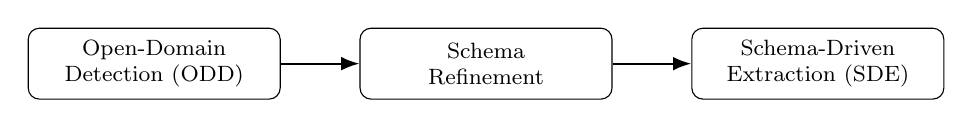
\begin{tikzpicture}[
  node distance=10mm,
  box/.style={draw, rounded corners, minimum height=9mm, minimum width=32mm, align=center, font=\footnotesize},
  arr/.style={-Latex, thick}
]
  \node[box] (det) {Open-Domain\\Detection (ODD)};
  \node[box, right=of det] (onto) {Schema\\Refinement};
  \node[box, right=of onto] (extr) {Schema-Driven\\Extraction (SDE)};
  \draw[arr] (det) -- (onto);
  \draw[arr] (onto) -- (extr);
\end{tikzpicture}
  }
\caption{Extraction pipeline inspired by ODKE+.}
\label{fig:extraction}
\end{figure}

\subsubsection{Open-Domain Detection (ODD)}
The goal of the first step is to discover, from the document, which entity types and relation types are meaningful. Text is split using a recursive characters splitter with a chunk size of {1200 characters and an overlap of 200 characters}~\cite{shereshevsky2026}. The relatively larger window is used deliberately: at this stage the GPT-5.4-mini model is asked about types, not instances, and a wider context helps it see more than one sentence at a time, which is important in legal language, where a concept such as \textit{tax base} is often introduced several sentences before it is first used. Each chunk $c_i$ is sent in parallel to an agent whose system prompt instructs it to return generic but distinguishable node labels and relationship labels, with an explicit focus on laws, paragraphs, obligations, rights and temporal entities. All Slovak diacritics are normalised to ASCII so that the graph uses a single consistent spelling. The output of this step is a list of per-chunk schemas $S_i=(\mathcal{T}^{(i)}_V,\mathcal{T}^{(i)}_E)$. For next step, the per-chunk schemas are merged into a single united set of node types and relation types: $S_{\text{ODD}}=\bigcup_{i=1}^{|C|} S_i $

\subsubsection{Schema Refinement (SR)}
The merged schema from ODD is sent to a schema refinement using Gemini 2.5 Pro call together with any existing ontology already stored in graph: $S^{\ast}=\Phi(S_{\text{ODD}},\,S_0)$. The refinement step has a clear linguistic role: it resolves duplicates caused by diacritics or minor spelling variants (for example Dan vs Daň), and semantically similar types (for example \textit{Doklad}, \textit{DanovyDoklad} and \textit{HodnovernyDoklad} into \textit{Doklad}). It enforces upper-snake-case for relation types and it refuses to merge semantically distinct categories such as \textit{Document} (\textit{Dokument}) and \textit{Person} (\textit{Osoba}). A merge log is kept that maps every canonical type back to the raw variants it absorbed, which is useful both for debugging and for auditing. A special type \textit{Paragraph} is always added to the node list, because every legal fact in the graph should be traceable back to the paragraph that states it.

\begin{figure*}[t]
\centering

\begin{minipage}[t]{0.48\textwidth}
  \centering
  \scalebox{0.60}{%
  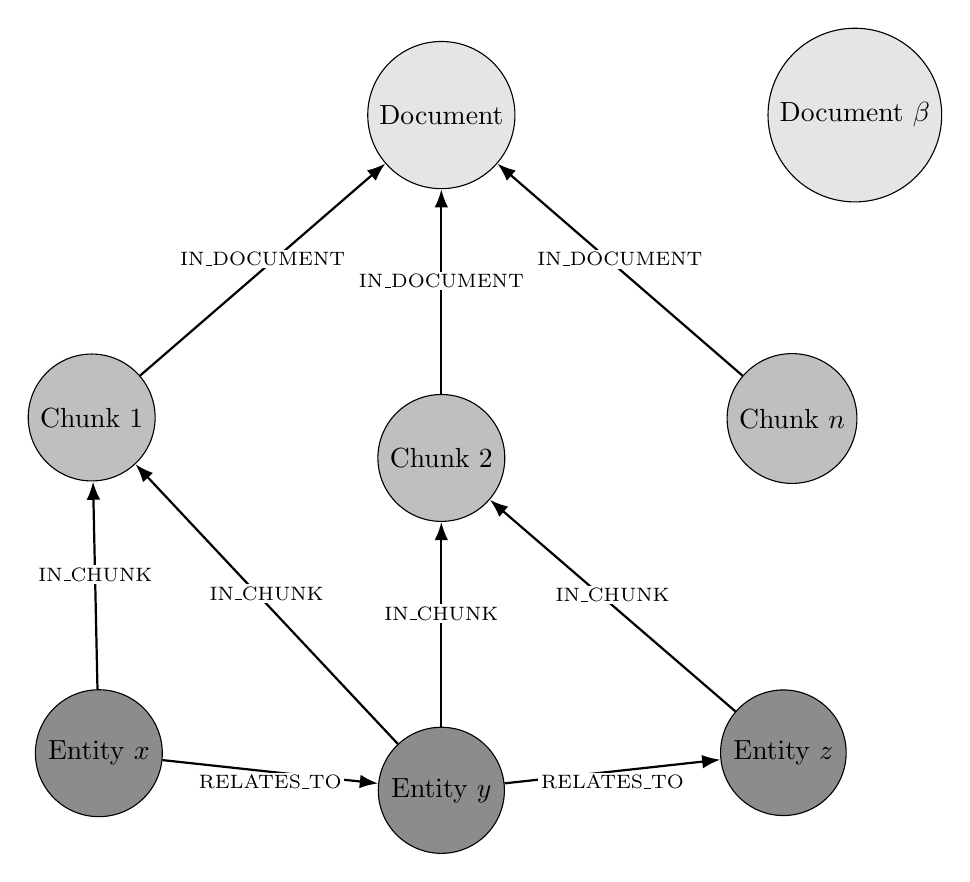
\begin{tikzpicture}[
    node distance=26mm and 32mm,
    doc/.style={circle, draw, fill=gray!20, minimum size=14mm, align=center},
    chunk/.style={circle, draw, fill=gray!50, minimum size=14mm, align=center},
    ent/.style={circle, draw, fill=gray!90, minimum size=14mm, align=center},
    arr/.style={-Latex, thick}
  ]
    \node[doc] (doc) {Document};
    \node[doc, right=of doc] (doc2) {Document $\beta$};

    \node[chunk, below left=of doc] (c1) {Chunk 1};
    \node[chunk, below=of doc] (c2) {Chunk 2};
    \node[chunk, below right=of doc] (cn) {Chunk $n$};

    \node[ent, below left=of c2] (ex) {Entity $x$};
    \node[ent, below=of c2] (ey) {Entity $y$};
    \node[ent, below right=of c2] (ez) {Entity $z$};

    \draw[arr] (c1) -- node[midway, above, fill=white, inner sep=1pt]{\scriptsize IN\_DOCUMENT} (doc);
    \draw[arr] (c2) -- node[midway, above, fill=white, inner sep=1pt]{\scriptsize IN\_DOCUMENT} (doc);
    \draw[arr] (cn) -- node[midway, above, fill=white, inner sep=1pt]{\scriptsize IN\_DOCUMENT} (doc);

    \draw[arr] (ex) -- node[midway, above, fill=white, inner sep=1pt]{\scriptsize IN\_CHUNK} (c1);
    \draw[arr] (ey) -- node[midway, above, fill=white, inner sep=1pt]{\scriptsize IN\_CHUNK} (c1);
    \draw[arr] (ey) -- node[midway, above, fill=white, inner sep=1pt]{\scriptsize IN\_CHUNK} (c2);
    \draw[arr] (ez) -- node[midway, above, fill=white, inner sep=1pt]{\scriptsize IN\_CHUNK} (c2);

    \draw[arr] (ex) -- node[midway, below, fill=white, inner sep=1pt]{\scriptsize RELATES\_TO} (ey);
    \draw[arr] (ey) -- node[midway, below, fill=white, inner sep=1pt]{\scriptsize RELATES\_TO} (ez);
  \end{tikzpicture}
  }
  \captionof{figure}{{Knowledge graph structure: document, chunk, entity and relationships. Image taken and edited to our solution from Neo4j}~\cite{neo4jblog}}
  \label{fig:graph_structure}
\end{minipage}%
\hfill
\begin{minipage}[t]{0.48\textwidth}
  \centering
  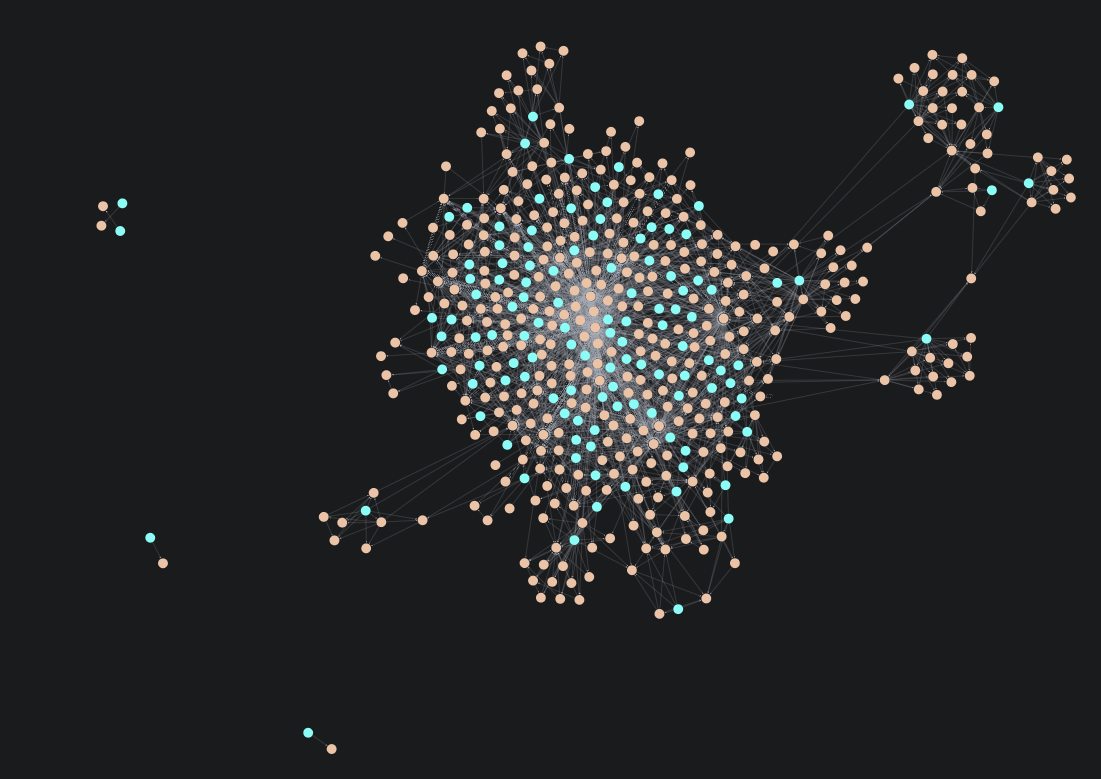
\includegraphics[width=\linewidth]{../grafova_databaza.png}
  \captionof{figure}{Graph database in Neo4j Desktop.}
  \label{fig:dual_db}
\end{minipage}

\end{figure*}

\subsubsection{Schema-Driven Extraction (SDE)}
The final extraction step uses the refined $S^{\ast}$ schema as a hard constraint. Text is rechunked with a smaller window of {1024 characters and an overlap of 128 characters}~\cite{shereshevsky2026}. This smaller chunk is motivated by a different trade-off: at this stage the GPT-5.4-mini model must extract concrete instances and a shorter window pushes it to produce tighter, better-grounded triples $(e_h, r, e_t)$, where $e_h$ is head entity, $e_t$ is tail entity and $r$ is relationship between them. It reduces the chance that two unrelated facts are blended into one relation, and makes the per-chunk LLM cost predictable. The chunks are sent in parallel, with a bounded concurrency and an automatic pause-and-retry mechanism in case of provider errors (when user hits Tokens Per Minute limit). For each chunk $c_i$ the model returns nodes and relationships, that conform to the refined $S^{\ast}$ schema and yields a GraphDocument $G_i = (V_i, E_i, src_i)$. A lightweight post-processing step normalises node IDs to title case, normalises relation names to upper-snake-case, and drops entries with missing source or target. Every extracted node is also linked to a \textit{Chunk} node via an IN\_CHUNK relation, which later allows retrieval stage to fetch the original text that supports a given triple.




\subsection{Database Insertion}
Extracted graph documents are inserted into a {Neo4j database}~\cite{neo4j}. Nodes are created with MERGE on their normalised ID so that repeated mentions across chunks collapse into a single entity. Relationships are created in the same MERGE style to avoid duplicate edges. In addition to the extracted nodes and edges, the pipeline also inserts a Document node per source PDF, linked to every Chunk node via an IN\_DOCUMENT relation.

\section{Search and Retrieval}
The query pipeline follows {KG-GPT framework}~\cite{kggpt2023}: sentence segmentation, graph retrieval and inference. Fig.~\ref{fig:qeury} summarises the flow.

\begin{figure}[h]
\centering
  \scalebox{0.75}{%
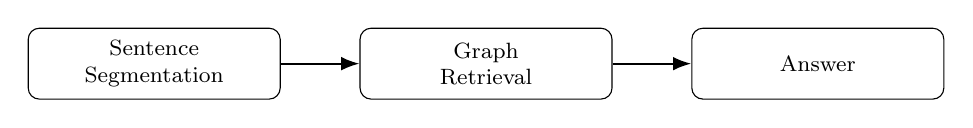
\begin{tikzpicture}[
  node distance=10mm,
  box/.style={draw, rounded corners, minimum height=9mm, minimum width=32mm, align=center, font=\footnotesize},
  arr/.style={-Latex, thick}
]
  \node[box] (det) {Sentence\\Segmentation};
  \node[box, right=of det] (onto) {Graph\\Retrieval};
  \node[box, right=of onto] (extr) {Answer};
  \draw[arr] (det) -- (onto);
  \draw[arr] (onto) -- (extr);
\end{tikzpicture}
  }
  \caption{Query pipeline. Each sub-sentence is retrieved independently.}
\label{fig:qeury}
\end{figure}

\subsection{Sentence Segmentation}
Legal question are often compound. A single question such as "which paragraph of the law defines the tax base and what is the formula used to compute it" implies two graph facts, not one. The segmentation stage, following the approach of KG-GPT~\cite{kggpt2023}, breaks the user question into sub-sentences and for each sub-sentence, extracts up to two anchor entities written in title case. Every sub-sentence is meant to correspond to approximately one graph triple $(e_h, r, e_t)$. The returned object is $(\text{sentence}_j,\ \text{entities}_j)$ If no sub-sentence is produced, the original question is used as a fallback.

\subsection{Graph Retrieval}
The middle stage is the most sensitive part of the pipeline, because it is where answers are grounded in actual graph evidence. We implement an agent inspired by {ARK-V1}~\cite{arkv12025}. For each sub-sentence, and for each anchor entity mentioned in it (up to two), the agent performs a bounded walk of depth at most $K_{max} = 3$.

A single step of the chain has four internal sub-steps. First, the anchor is resolved: the graph is queried for a node whose ID matches case-insensitively, or as a fallback contains the raw anchor string. Second, all relation types actually incident to the resolved anchor are enumerated, both outgoing and incoming. This produces the candidate set $R^k$. Third, the LLM is asked to pick exactly one relation from $R^k$ or to return null. The prompt is rebuilt from scratch at every step and contains only the system instruction, the sub-sentence, the current anchor, the running summary and the candidate list. This keeps context size roughly constant in $k$. Up to $C_{max} = 2$ retries are allowed, and the choice is validated against $R^k$ on every retry. Fourth, triples of the form $(e_{anchor}, rel, u)$, where $u$ is any entity, are enumerated from the graph, capped at 25 per step, and the LLM selects the relevant indices, summarization the implication of the step and decides whether to continue. If it continues, a tail of one of the selected triples becomes the new anchor and the loop repeats.

Formally, at step $k$ the agent maintains the state $s_k = (a_k, \Sigma_k, E_k)$, where $a_k$ is the current anchor, $\Sigma_k$ is the running textual summary and $E_k$ is the accumulated set of evidence triples. The transition picks a relation $r_k \in R^k$ and a subset of triples $T_k \subseteq \{(a_k, r_k, t): t \in V\}$. The update is 

$$
E_{k+1} = E_k \cup T_k, \qquad a_{k+1} \in \pi_3(T_k) \cup \{a_k\},
$$

where $\pi_3$ projects a triple onto its tail. The chain terminates when the agent sets the \textit{continue} flag to false, when $R^k$ is empty or when $k$ reaches $K_{max}$

Two design choices important noticing. First, the candidate set $R^k$ is always built from the graph itself. This means the agent can never propose a relation that does not exist for the current anchor, which eliminates an entire class of hallucinations. Second, the running summary $\Sigma_k$ is the only long-term memory carried between steps. The triples themselves are re-enumerated every time. This is what makes the context size predictable even for deep walks. At the end of the per-anchor loop the evidence triples are deduplicated while preserving insertion order.

\begin{figure}[t]
\centering
\scalebox{0.55}{%
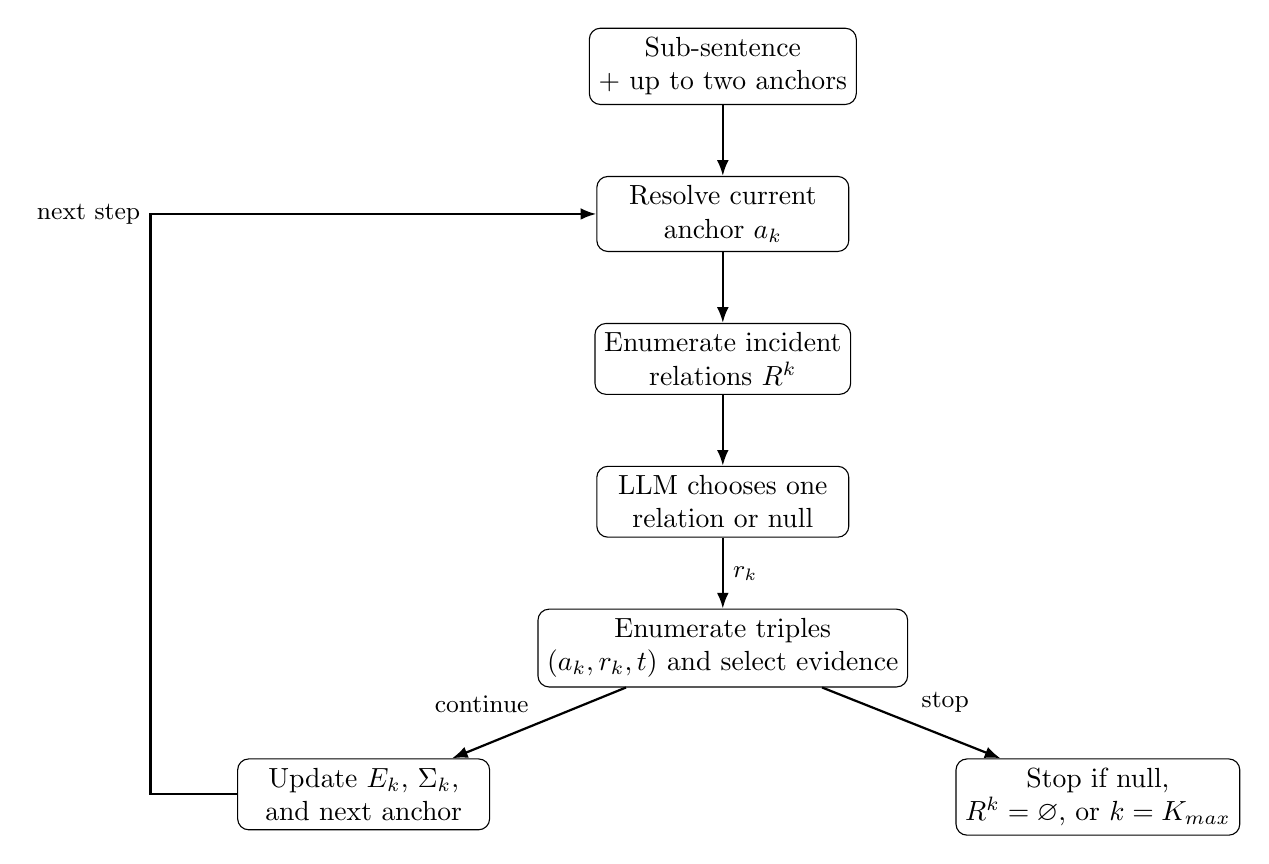
\begin{tikzpicture}[
    node distance=9mm and 8mm,
    box/.style={draw, rounded corners, align=center, minimum width=3.2cm, minimum height=9mm},
    line/.style={-{Latex[length=2mm]}, thick}
]
    \node[box] (query) {Sub-sentence\\+ up to two anchors};
    \node[box, below=of query] (resolve) {Resolve current\\anchor $a_k$};
    \node[box, below=of resolve] (relations) {Enumerate incident\\relations $R^k$};
    \node[box, below=of relations] (choose) {LLM chooses one\\relation or null};
    \node[box, below=of choose] (triples) {Enumerate triples\\$(a_k,r_k,t)$ and select evidence};
    \node[box, below left=of triples, xshift=2mm] (update) {Update $E_k$, $\Sigma_k$,\\and next anchor};
    \node[box, below right=of triples, xshift=-2mm] (stop) {Stop if null,\\$R^k=\varnothing$, or $k=K_{max}$};

    \draw[line] (query) -- (resolve);
    \draw[line] (resolve) -- (relations);
    \draw[line] (relations) -- (choose);
    \draw[line] (choose) -- node[right, font=\small] {$r_k$} (triples);
    \draw[line] (triples) -- node[above left, font=\small] {continue} (update);
    \draw[line] (triples) -- node[above right, font=\small] {stop} (stop);
    \draw[line] (update.west) |- ++(-1.1,0) |- node[left, font=\small] {next step} (resolve.west);
\end{tikzpicture}
}
\caption{Simple evidence-retrieval loop over the knowledge graph. For each anchor, the agent resolves the node, enumerates valid relations from the graph, chooses one relation, selects supporting triples, and either continues with a new anchor or stops.}
\label{fig:graph-retrieval-flow}
\end{figure}

\subsection{Inference}
The final stage aggregates the evidence triples from all sub-sentences into a single list and retrieves the text chunks linked to the involved nodes via the IN\_CHUNK relationship. A Gemini 2.5 Flash model is then prompted with three blocks: the original user question, retrieved evidence triples $(e_h, r, e_t)$ as primary evidence, and the retrieved chunks as supplementary context. The prompt instructs the model to prioritise the graph triples and to use the chunks only for wording and context. The output is a short Slovak answer grounded in explicit graph evidence.

\section{Conclusion}

We presented a GraphRAG pipeline tailored to Slovak financial law. On the construction side, layout-aware preprocessing preserves tables and formulas, and an ODKE+ inspired three-step extraction produces a stable ontology with chunk-level provenance. On the query side, a KG-GPT pipeline with an ARK-V1-inspired agent in the middle stage walks the graph in small, verifiable hops and grounds every answer in explicit evidence. Future work includes a quantitative evaluation on a curated set of Slovak legal questions


\section*{Acknowledgment}

This research was done with support of projects VEGA 1/0800/16 INOMET and H2020 NEWTON Ref. No.: 688503. I declare that generative artificial intelligence tool, OpenAI \url{prism.openai.com}, GPT-5.4 (2026), was used to generate graph material in this paper. 

\begin{thebibliography}{00}

\bibitem{yao2024}
Y. Yao, J. Duan, K. Xu, Y. Cai, Z. Sun, and Y. Zhang, ``A survey on large language model (LLM) security and privacy: The good, the bad, and the ugly,'' \textit{High-Confidence Computing}, vol.~4, no.~2, 2024, Art.\ no.\ 100211.

\bibitem{neo4j}
Neo4j, Inc., ``Neo4j graph database.'' [Online]. Available: \url{https://neo4j.com/}

\bibitem{odkeplus2025}
S. Khorshidi \textit{et al.}, ``ODKE+: Ontology-guided open-domain knowledge extraction with LLMs,'' arXiv preprint arXiv:2509.04696, 2025. [Online]. Available: \url{https://arxiv.org/abs/2509.04696}

\bibitem{kggpt2023}
J. Kim, Y. Kwon, Y. Jo, and E. Choi, ``KG-GPT: A general framework for reasoning on knowledge graphs using large language models,'' in \textit{Findings of the Association for Computational Linguistics: EMNLP 2023}, Singapore, Dec.\ 2023, pp.\ 9410--9421. [Online]. Available: \url{https://aclanthology.org/2023.findings-emnlp.631/}

\bibitem{arkv12025}
J.-F. Klein and L. Ohnemus, ``ARK-V1: An LLM-agent for knowledge graph question answering requiring commonsense reasoning,'' arXiv preprint arXiv:2509.18063, 2025. [Online]. Available: \url{https://arxiv.org/abs/2509.18063}

\bibitem{langchain}
LangChain, Inc., ``LangChain documentation.'' [Online]. Available: \url{https://docs.langchain.com/}

\bibitem{edge2024}
D. Edge \textit{et al.}, ``From local to global: A Graph RAG approach to query-focused summarization,'' arXiv preprint arXiv:2404.16130, 2024. [Online]. Available: \url{https://arxiv.org/abs/2404.16130}

\bibitem{knobuilder2025}
B. J. Serrano Mena, ``KnoBuilder: An LLM-agent for autonomous and personalized knowledge graph construction from unstructured text,'' in \textit{Proc.\ NeurIPS}, 2025. [Online]. Available: \url{https://openreview.net/forum?id=teewCPCv2m}

\bibitem{graphjudge2025}
H. Huang, C. Chen, Z. Sheng, Y. Li, and W. Zhang, ``Can LLMs be good graph judge for knowledge graph construction?,'' in \textit{Proc.\ 2025 Conf.\ Empirical Methods in Natural Language Processing (EMNLP)}, Suzhou, China, Nov.\ 2025, pp.\ 10929--10948. [Online]. Available: \url{https://aclanthology.org/2025.emnlp-main.554/}

\bibitem{rwt2025}
T. Shen, J. Wang, X. Zhang, and E. Cambria, ``Reasoning with trees: Faithful question answering over knowledge graph,'' in \textit{Proc.\ 31st Int.\ Conf.\ Computational Linguistics (COLING)}, Abu Dhabi, UAE, Jan.\ 2025, pp.\ 3138--3157. [Online]. Available: \url{https://aclanthology.org/2025.coling-main.211/}

\bibitem{gmello2024}
R. Chen \textit{et al.}, ``LLM-based multi-hop question answering with knowledge graph integration in evolving environments,'' arXiv preprint arXiv:2408.15903, 2024. [Online]. Available: \url{https://arxiv.org/abs/2408.15903}

\bibitem{lightrag2024}
Z. Guo, L. Xia, Y. Yu, T. Ao, and C. Huang, ``LightRAG: Simple and fast retrieval-augmented generation,'' arXiv preprint arXiv:2410.05779, 2024. [Online]. Available: \url{https://arxiv.org/abs/2410.05779}

\bibitem{legograph2024}
Y. Cao, Z. Gao, Z. Li, X. Xie, S. K. Zhou, and J. Xu, ``LEGO-GraphRAG: Modularizing graph-based retrieval-augmented generation for design space exploration,'' arXiv preprint arXiv:2411.05844, 2024. [Online]. Available: \url{https://arxiv.org/abs/2411.05844}

\bibitem{das2024}
B. C. Das, M. H. Amini, and Y. Wu, ``Security and privacy challenges of large language models: A survey,'' \textit{ACM Comput.\ Surv.}, vol.~57, no.~6, 2025. Also available as arXiv:2402.00888. [Online]. Available: \url{https://arxiv.org/abs/2402.00888}

\bibitem{neo4jblog}
E. Kohlwey, ``GraphRAG field guide: Navigating the world of advanced RAG patterns,'' \textit{Neo4j Developer Blog}, 2024. [Online]. Available: \url{https://neo4j.com/blog/developer/graphrag-field-guide-rag-patterns/}

\bibitem{shereshevsky2026}
A. Shereshevsky, ``Building knowledge graphs from Homer's Iliad: Open-domain vs.\ schema-guided extraction,'' \textit{Graph \& Quill, Medium}, Jan.\ 2026. [Online]. Available: {\def\UrlBreaks{\do\/\do\-\do\.}\Urlmuskip=0mu plus 1mu\relax\url{https://medium.com/graph-quill/building-knowledge-graphs-from-homers-iliad-open-domain-vs-schema-guided-extraction-ef0bf3874a33}}

\end{thebibliography}

\end{document}